\documentclass[10pt]{beamer}

% Package
\usepackage{graphicx}
\usepackage{tcolorbox}
\usepackage{listings}

% Theme
\usetheme{Warsaw}
\usecolortheme{beaver}

% Main & Info
\title[Angular]
{Module Angular}
\subtitle{Partie 1}
\author[Maxime Tournier]
{Maxime Tournier}
\date[21/08/2023]

% Start
\begin{document}

	\frame{\titlepage}

	\begin{frame}
		\frametitle{Sommaire}

		1. {Présentation} \newline
		2. {Histoire} \newline
		3. {Démarrage Angular} \newline
		4. {TypeScript} \newline
		4. {Premier pas sur Angular} \newline
		5. {Composants} \newline
		6. {Template} \newline

	\end{frame}

%%%%%%%% Présentation

	\begin{frame}
		\frametitle{Présentation}
	
		Angular est un \alert{FrameWork}

		\begin{block}{Traduction}
			Framework = Cadre de travail
		\end{block}

		En tant que développeur, on fait souvent la même chose \newline \newline
		Exemple: \newline Valider les formulaires | Gérer la navigation | Traiter les erreurs
		\newline \newline
		Et pour régler ce problème au lieu d'aller récupéré les fonctions d'autres projet on a créé les frameworks
		\newline \newline
		Avantage : Tout le monde travaille sur les mêmes fonctions
		
	\end{frame}

	\begin{frame}
		\frametitle{Présentation}

		Pour comprendre le fonctionnement d'angular
		\newline \newline
		Il faut comprendre le web aujourd'hui
		\newline \newline
		Site Web / Application Web
		\newline \newline
		Il s'agit bien de deux choses différentes

	\end{frame}

	\begin{frame}
		\frametitle{Présentation}

		Avant ça comment ça marche :

			
\includegraphics[width=2cm]{assets/page}\newline
			- Fichier client (CSS, HTML, JS)

			
\includegraphics[width=2cm]{assets/server}\newline
			- Fichier serveur (php, java) (ici qu'on fait des requêtes sql)

	\end{frame}

	\begin{frame}
		\frametitle{Présentation}

		Et donc un site web fonctionne comme ça :
		\newline \newline

		\centering
		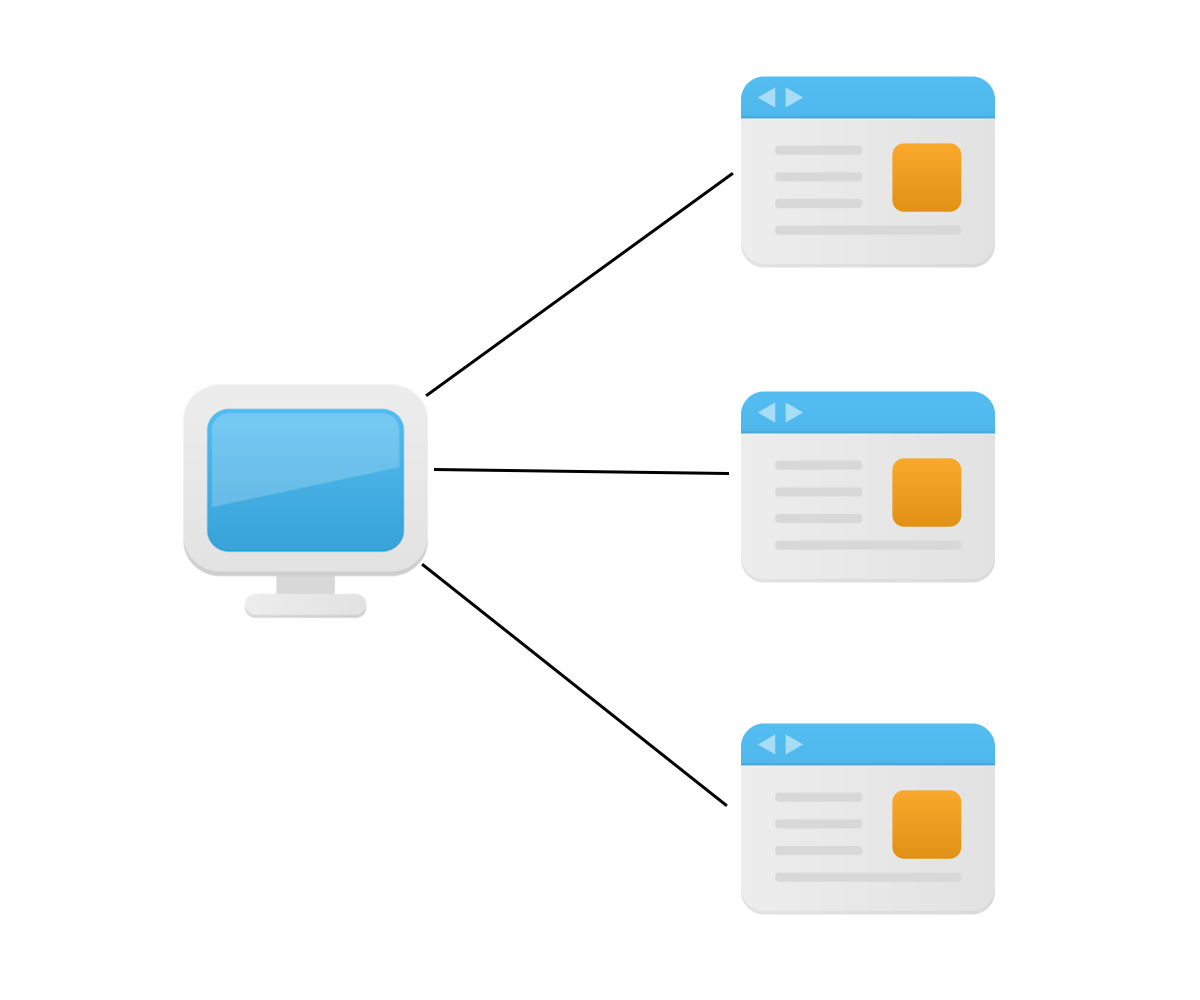
\includegraphics[width=6cm]{assets/siteweb}\newline

	\end{frame}

	\begin{frame}
		\frametitle{Présentation}

		Et une application web marche comme ça:
		\newline \newline

		\centering
		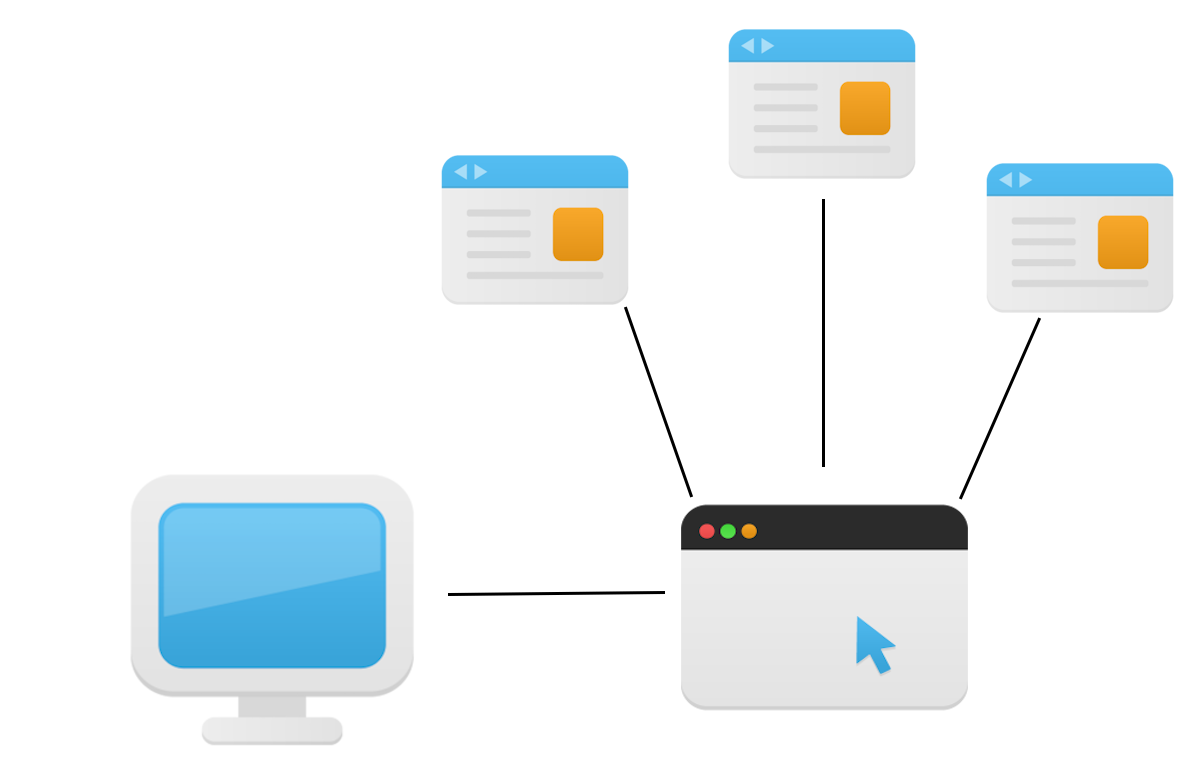
\includegraphics[width=8cm]{assets/appweb}\newline

	\end{frame}

	\begin{frame}
		\frametitle{Présentation}

		Resumé :
		\newline \newline
		le client doit faire une requête au serveur a chaque fois dans un site web \newline \newline
		alors que dans une application web, nous allons déléguer le travaille à Javascript qui va désactiver ou activer une partie du code html/css
		\newline \newline
		\begin{block}{Information}
			Cette méthode s'appelle SPA (Single Page Application)
		\end{block}
	\end{frame}

%%%%%%%% Histoire

	\begin{frame}
		\frametitle{Histoire}

		AngularJS n'est pas égal à Angular \newline \newline

		AngularJS a été créé par Google \newline \newline

		AngularJS avait comme architecture MVC \newline \newline

		AngularJS n'est plus maintenu depuis 2018 \newline \newline

		\begin{block}{MVC}
			Module Vue Controlleur (Comme Symfony)
		\end{block}

	\end{frame}

	\begin{frame}
		\frametitle{Histoire}

		Angular est un framework orienté composant \newline \newline

		Nous allons coder une multitude de petits composants qui formera une application \newline \newline

		Un composant est une partie du site qui fonctionne de manière autonome sur une application

	\end{frame}

	\begin{frame}
		\frametitle{Histoire}

		Angular est-il difficile à apprendre ? : \newline \newline

		Angular a une réputation de framework difficile \newline \newline

		Car Angular est basé sur Typescript une langue basée sur Javascript qui permet de Typé vos variables \newline \newline

		Angular est basé sur la version de Javascript ES6

	\end{frame}

	\begin{frame}
		\frametitle{Information}
		\centering
		Regarder la documentation
		S'IL VOUS PLAIT

		Angular.io

	\end{frame}

%%%%%%%% Demarrage Angular

	\begin{frame}
		\frametitle{Démarrage Angular}

		1. Installer un environnement de développement \newline
		2. Génère un socle angular (Grâce à Angular-CLI)\newline
		3. Nous allons jouer avec le composant racine =)
		\newline \newline
		\begin{block}{Information}
			un composant c’est comme une partie de l’application web. Mais il y a un premier composant à l'origine de tout, que nous appelons le composant racine
		\end{block}

	\end{frame}

	\begin{frame}
		\frametitle{Démarrage Angular}

		Ce qu'on a besoin : \newline \newline

		D'abors on va avoir besoin du moteur javascript (NodeJS) et d'un gestionnaire de paquets (NPM) \newline \newline

		D'un éditeur de code TypeScript \newline \newline

		Un outil qu'on appelle Angular CLI (Qui va nous permet de gérer notre projet Angular)

	\end{frame}

	\begin{frame}
		\frametitle{NodeJS et NPM}

		NodeJS et NPM sont utilisés pour la majorité des projets Javascript moderne \newline \newline

		NodeJS permet d’excuter du code JS côté serveur \newline \newline

		NPM permet de géré les dépence de paquet de javascript (angular est un paquet) \newline \newline

		NodeJS intègre par défaut NPM

	\end{frame}

	\begin{frame}
		\frametitle{NodeJS et NPM}

		Pour installer NodeJS (et donc aussi NPM) \newline \newline

		il vous suffit d'installer sur le site officiel https://nodejs.org/fr \newline \newline

		\begin{block}{Information}
			Prenez la version LTS
		\end{block}

	\end{frame}

	\begin{frame}
		\frametitle{IDE}

		On va avoir besoin d'un IDE \newline \newline

		Un IDE est un environnement de développement (Editeur de code amélioré) \newline \newline

		- Visual Studio Code : Recommander par Mircorsoft (Gratuit) \newline
		- WebStorm :Beaucoup plus puissant et recommandés par Google, de la suite JetBrain (Payant) \newline  \newline

		Choisissez celui que vous préférez ou que vous êtes le plus à l'aise  \newline \newline

		\begin{block}{Information}
			La suite JetBrain (WebStorm) est gratuite pendant tout au long de votre formation, inscription sur leurs sites internet
		\end{block}

	\end{frame}

	\begin{frame}
		\frametitle{Terminal}

		Pour votre terminal : \newline \newline

		Souvent il peut avoir des problèmes avec le terminal Windows \newline \newline

		Essayer de toujours d'utiliser PowerShell \newline \newline

	\end{frame}

	\begin{frame}
		\frametitle{Démarrage Angular}

		Activité :  \newline \newline

		- Installer NodeJS et NPM sur le site officiel (https://nodejs.org/fr)
		Prenez la version LTS pour NodeJS  \newline \newline

		- Installer un IDE : Visual Studio Code ou WebStorm  \newline \newline

		Pour tester si NodeJS et NPM son bien installer, Ouvrez un terminal  \newline
		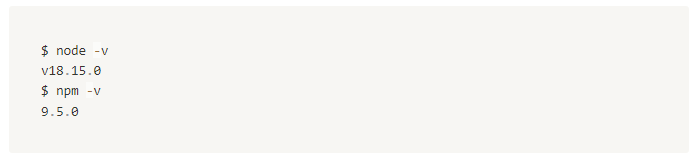
\includegraphics[width=10cm]{assets/npminstall}\newline

	\end{frame}

%%%%%%%% TypeScript

	\begin{frame}
		\frametitle{TypeScript}

		TypeScript est une surcouche de JavaScript  \newline \newline

		Typescript est développé par Microsoft depuis 2012  \newline \newline

		TypeScript support les dernier version de JS ES6

	\end{frame}

	\begin{frame}
		\frametitle{TypeScript}

		TypeScript a besoin d’être compilé (Build) pour fonctionner  \newline \newline

		Il sera transformé en un fichier JS  \newline \newline

		L’extension de TS est .ts

	\end{frame}

	\begin{frame}
		\frametitle{TypeScript}

		Pour compiler Typescript on exécutera cette commande \newline \newline


		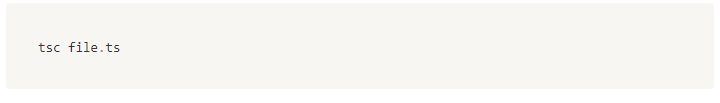
\includegraphics[width=15cm]{assets/tsbuild}\newline


		Cette commande nous créera un fichier JS du nom de file.js

	\end{frame}

	\begin{frame}
		\frametitle{TypeScript}

		Typescript ajoute la déclaration de variable: \newline \newline


		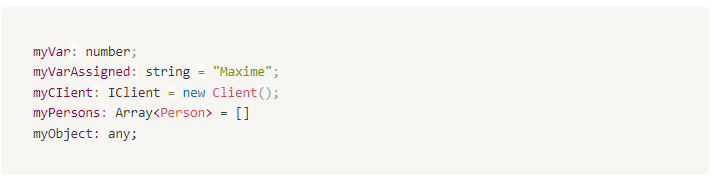
\includegraphics[width=15cm]{assets/tsvariable}\newline


	\end{frame}

	\begin{frame}
		\frametitle{TypeScript}

		Typescript ajoute la déclaration de variable: \newline \newline

		\centering
		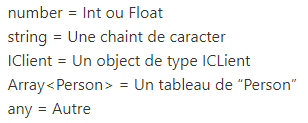
\includegraphics[width=7cm]{assets/tsvariable2}\newline


	\end{frame}


	\begin{frame}
		\frametitle{TypeScript}

		Activité : \newline \newline

		- Installer de quoi compile Typescript avec cette commande \newline \newline

		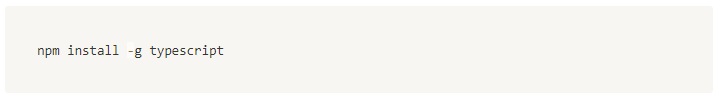
\includegraphics[width=16cm]{assets/tsInstall}\newline


	\end{frame}

	\begin{frame}
		\frametitle{TypeScript}

		Activité : \newline \newline

		- Refaire l'activité 1 du rappel JavaScript \newline
		En typant les variables avec Typescript \newline \newline

		- Puis compiler le fichier Typescript et tester le site \newline \newline



	\end{frame}

	\begin{frame}
		\frametitle{TypeScript}

		Activité : \newline \newline

		Mini-Quiz à Choix Multiples


	\end{frame}

%%%%%%%% Premier pas avec Angular

	\begin{frame}
		\frametitle{Premier pas avec Angular}

		Angular-CLI :  \newline \newline

		\centering
		Cette application va installer tout ce dont on a besoin \newline en une seul ligne de commande  \newline \newline

		et avec cette même outils on va pouvoir piloter certaines fonctionnalités d’angular directement en ligne de command  \newline \newline

		\begin{block}{Information}
			Ce n'est pas la seul méthode pour démarré un projet Angular, mais bien la plus connue
		\end{block}

	\end{frame}


	\begin{frame}
		\frametitle{Premier pas avec Angular}

		Activité : \newline \newline

		- Installer Angular-CLI  \newline \newline

		Grace à NPM :  \newline \newline

		npm install -g @angular/cli


	\end{frame}

	\begin{frame}
		\frametitle{Premier pas avec Angular}

		Activité : \newline \newline

		- Vérifier l'installation d'Angular-Cli  \newline \newline

		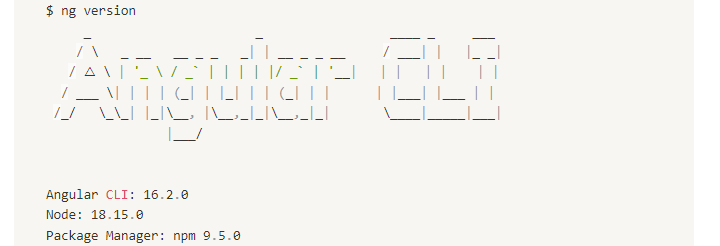
\includegraphics[width=16cm]{assets/angularCLInstall} \newline

		\begin{block}{Information}
			Toute les commandes d'angular-cli ce feront avec le prefix NG
		\end{block}

	\end{frame}

	\begin{frame}
		\frametitle{Premier pas avec Angular}

		Nous alons generez notre premier projet Angular \newline \newline

		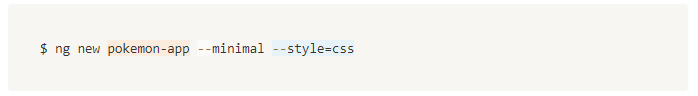
\includegraphics[width=16cm]{assets/angularsetup} \newline \newline

		Le nom du projet = pokemon-app \newline
		le type de ficher de style = css

	\end{frame}


	\begin{frame}
		\frametitle{Premier pas avec Angular}

		Activité : \newline
		Créer notre projet Angular \newline \newline

		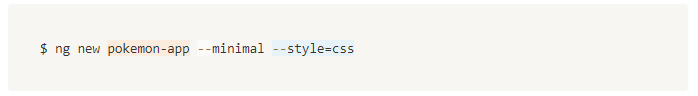
\includegraphics[width=17cm]{assets/angularsetup} \newline \newline

	\end{frame}

	\begin{frame}
		\frametitle{Premier pas avec Angular}

		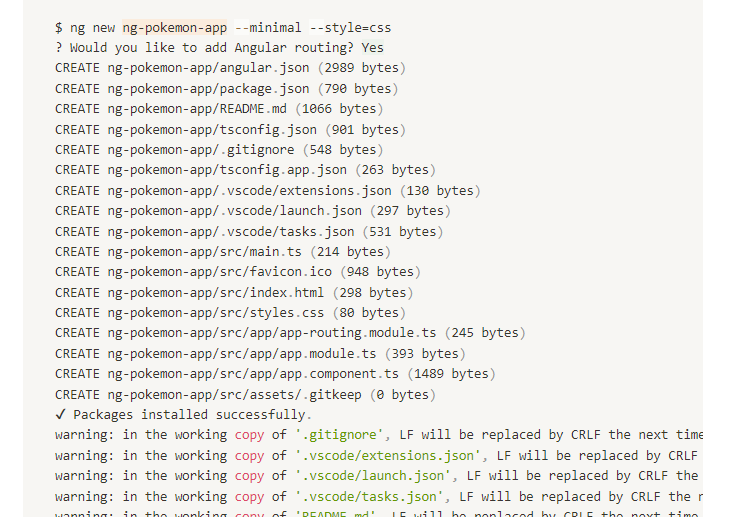
\includegraphics[width=15cm]{assets/angularsetup2} \newline \newline

	\end{frame}

	\begin{frame}
		\frametitle{Premier pas avec Angular}

		Que fait "Ng New" \newline \newline

		- Il créer tout le socle d'Augular\newline
		- Il installe toute les dépendance d'Angular (Il effectue des simple NPM INSTALL)\newline
		- Il initialise un .git \newline
		- Setup des confugurations pour des IDE\newline

	\end{frame}

	\begin{frame}
		\frametitle{Premier pas avec Angular}

		\centering
		Présentation du socle \newline \newline

	\end{frame}

	\begin{frame}
		\frametitle{Premier pas avec Angular}

		Lancé Angular : \newline \newline

		\centering
		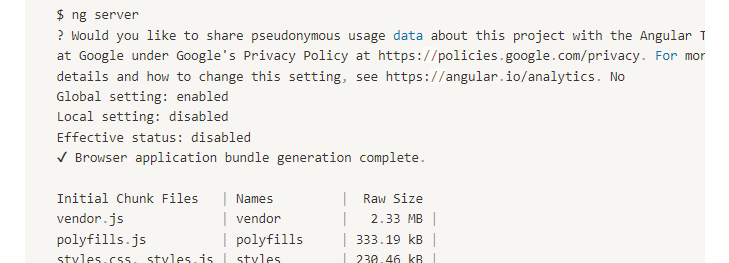
\includegraphics[width=15cm]{assets/ngserve} \newline

	\end{frame}

	\begin{frame}
		\frametitle{Premier pas avec Angular}

		\centering
		Inspection premier composant \newline \newline

	\end{frame}

	\begin{frame}
		\frametitle{Premier pas avec Angular}

		\centering
		Inspection du module racine \newline \newline

	\end{frame}

	\begin{frame}
		\frametitle{Premier pas avec Angular}

		\centering
		Configuration TypeScript \newline \newline


		\centering
		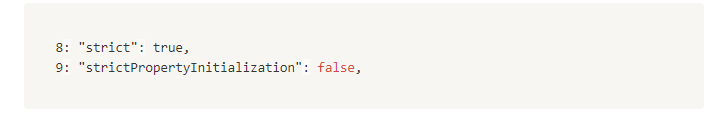
\includegraphics[width=11cm]{assets/tsConfig} \newline

	\end{frame}

%%%%%%%% Composant

	\begin{frame}
		\frametitle{Composants}

		Quest-ce qu'un composants ? : \newline \newline

		Un composants est une parti de l'écran \newline \newline

		Cette portion de l’écran qu’on vas controller,\newline on appel ça une vue  (ligne 5) \newline \newline

		cette vue est deffini dans le template et ça peut-etre beaucoup chose \newline \newline

		Donc un composant est une class + une vue
	\end{frame}

	\begin{frame}
		\frametitle{Composants}

		Quest-ce qu'un composants ? : \newline \newline

		le template (la vue) c'est le rendu pour les utilisateurs

		\centering
		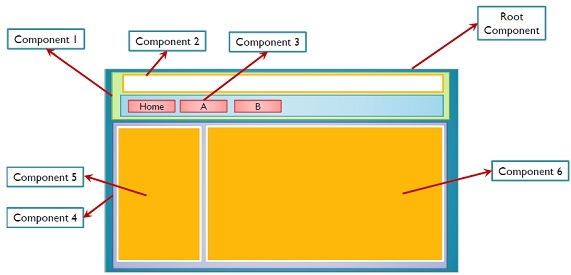
\includegraphics[width=11cm]{assets/composant} \newline


	\end{frame}

	\begin{frame}
		\frametitle{Composants}

		Première variable : \newline \newline

		\centering
		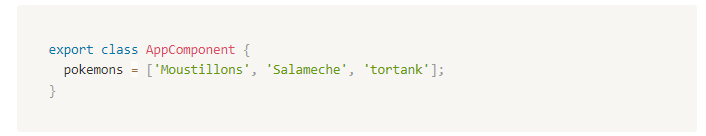
\includegraphics[width=11cm]{assets/tableauComposant} \newline

	\end{frame}

	\begin{frame}
		\frametitle{Composants}

		Activité : \newline \newline

		Afficher un pokémon dans votre template !

	\end{frame}

	\begin{frame}
		\frametitle{Composants}

		Affichage de notre première variable : \newline \newline

		\centering
		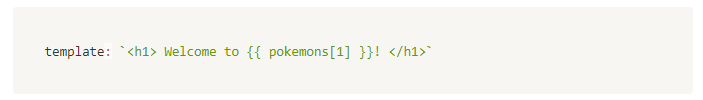
\includegraphics[width=11cm]{assets/templateComposant} \newline

	\end{frame}


	\begin{frame}
		\frametitle{Composants}

		Activité : \newline \newline

		- Créer deux variable de type number \newline
		- Mettez deux nombre aléatoire \newline
		- Afficher dans le template le resultat de l'addition de ces deux nombre \newline \newline


		\begin{block}{Information}
			Pensez a typé vos variable
		\end{block}

	\end{frame}

	\begin{frame}
		\frametitle{Composants}

		Cycle de vie : \newline

		\centering
		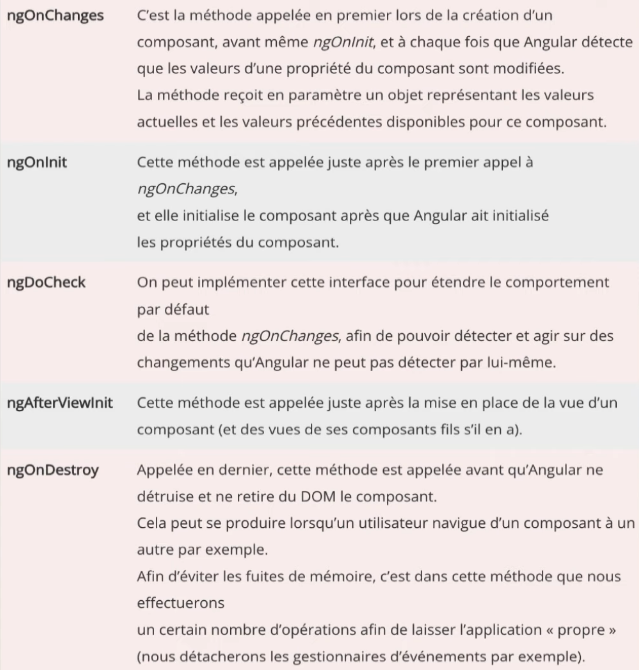
\includegraphics[width=7cm]{assets/vie} \newline


	\end{frame}

	\begin{frame}
		\frametitle{Composants}

		NgOnInit : \newline \newline

		On vas en chargant ce composont \newline vouloir afficher le tableau pokemon dans un console.log \newline \newline

		On vas devoir importé la fonctionnalité nessesaire  \newline \newline


	\end{frame}

	\begin{frame}
		\frametitle{Composants}

		NgOnInit : \newline \newline


		\centering
		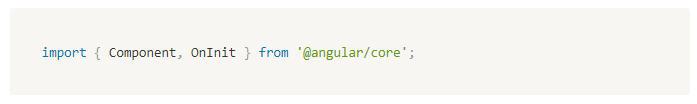
\includegraphics[width=11cm]{assets/ngoninit1} \newline


	\end{frame}

	\begin{frame}
		\frametitle{Composants}

		NgOnInit : \newline \newline


		\centering
		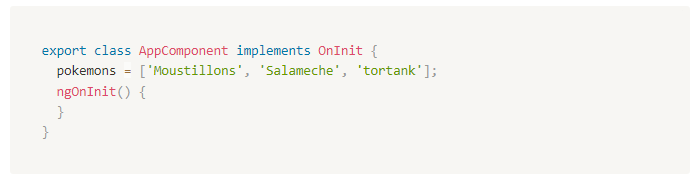
\includegraphics[width=11cm]{assets/ngoninit2} \newline


	\end{frame}

	\begin{frame}
		\frametitle{Composants}

		\centering
		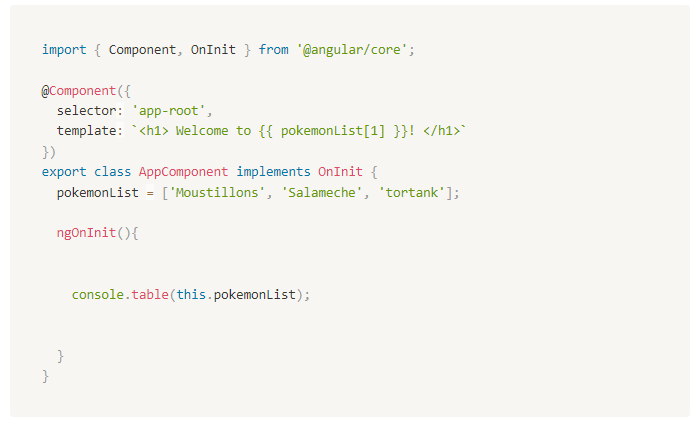
\includegraphics[width=12cm]{assets/consoleTable} \newline


	\end{frame}

	\begin{frame}
		\frametitle{Composants}

		Activité : \newline \newline

		- Créer une alert (Function JavaScript) au démarrage \newline
		- Cette alert dira "bonjour" au Utilisateur \newline \newline
		- Puis faite un "console.log" d'une nouvelle variable de type String \newline
		- La variable dira "Vous n'est pas polie" \newline \newline
		- Afficher dans un console.log l'additions de l'activité precedente

	\end{frame}

	\begin{frame}
		\frametitle{Composants}

		Interaction Utilisateur : \newline \newline

		On vas simplement créer une function qui affiche notre pokémon dans la console \newline \newline

		Une fois cette fonctionne créer, on vera dans le template comment activé cette fonction


	\end{frame}

	\begin{frame}
		\frametitle{Composants}

		Interaction Utilisateur : \newline \newline


		\centering
		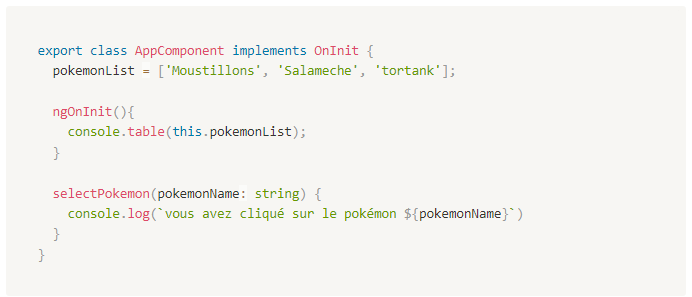
\includegraphics[width=12cm]{assets/userInt} \newline


	\end{frame}

	\begin{frame}
		\frametitle{Composants}

		Interaction Utilisateur : \newline \newline

		Pour tester cette fonction sans le template, on vas lancer la fonction au lancement du composant

		\centering
		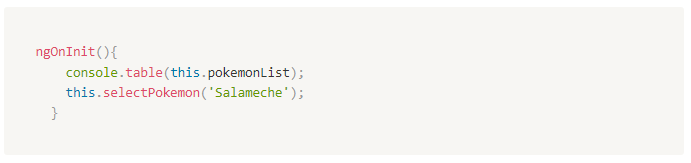
\includegraphics[width=12cm]{assets/userInt2} \newline


	\end{frame}

	\begin{frame}
		\frametitle{Composants}

		Activité : \newline \newline

		- Créer simplement une fonction "showId" \newline
		- qui aura comme argument "id" de type string \newline
		- et qui fera simplement un console.log d'"ID"

	\end{frame}

	\begin{frame}
		\frametitle{Composants}

		Activité : \newline \newline

		- Créer une fonction "multiplication" \newline
		- Cette fonction besoin de deux variable number pour foncitonner \newline
		- Cette fonction doit multiplier les deux variable et l'afficher dans un console.log \newline

		- Créer cette fonction et lancé la fonciton au démarrage du composant \newline en utilisant les deux variable "data1" et "data2"


	\end{frame}

	\begin{frame}
		\frametitle{Composants}

		Gerez de la donnée : \newline \newline

		nous allons créer deux fichier \newline \newline

		- ./src/app/pokemons.ts \newline
		- ./src/app/mock-pokemons-list.ts \newline \newline

		Le premier est un model (Class D'Object en php) \newline \newline

		Le Deuxième un tableau basé sur le model qui contient de la donnée

	\end{frame}

	\begin{frame}
		\frametitle{Composants}

		Activité : \newline \newline

		- Afficher en titre "Liste de pokémon" \newline
		- Recupéré dans la pokemonList toute les donnée du mock \newline
		- Dans la fonction selectPokemon recupéré tout un model pokémon plutot qu'un String \newline

	\end{frame}

%%%%%%%% Template
	\begin{frame}
		\frametitle{Template}

		Laisser la vue au même endroit que la logique \newline
		C'est absolument pas \alert{recommander} \newline \newline

		Alors dans notre composant on vas changer ça, \newline en créant un ficher appart\newline \newline

	\end{frame}

	\begin{frame}
		\frametitle{Template}

		On vas créer un fichier : \newline
		- ./src/app/app.component.html \newline \newline

		et modifier le composant : \newline


		\centering
		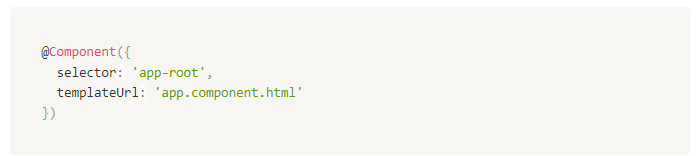
\includegraphics[width=12cm]{assets/templateAsset} \newline

	\end{frame}

	\begin{frame}
		\frametitle{Template}

		Dans app.component.html : \newline

		\centering
		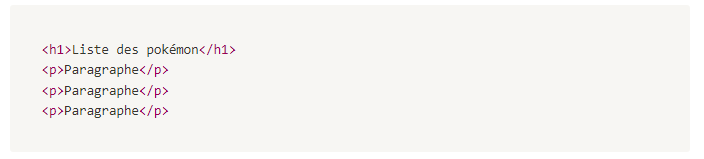
\includegraphics[width=14cm]{assets/templateHtml} \newline

	\end{frame}

	\begin{frame}
		\frametitle{Template}

		On peut constater que la vue ce charge bien par le biais de notre fichier html \newline \newline

		Et il y a bien toujours notre logique dans la console JavaScript  \newline \newline

		Donc maintenant on a fichier \alert{Logique} (Composant) et un fichier \alert{Graphique} (Template) \newline \newline

		c’est ce systeme qu’on vas utiliser tout au long du developpement Angular

	\end{frame}

	\begin{frame}
		\frametitle{Template}

		L'interpolation : \newline \newline

		Nous avons actuellement un fichier HTML \alert{static} \newline \newline

		Et nous voulons le rendre \alert{dynamique} \newline \newline

		On vas utiliser la syntaxe d’interpolation


	\end{frame}

	\begin{frame}
		\frametitle{Template}

		L'interpolation : \newline


		\centering
		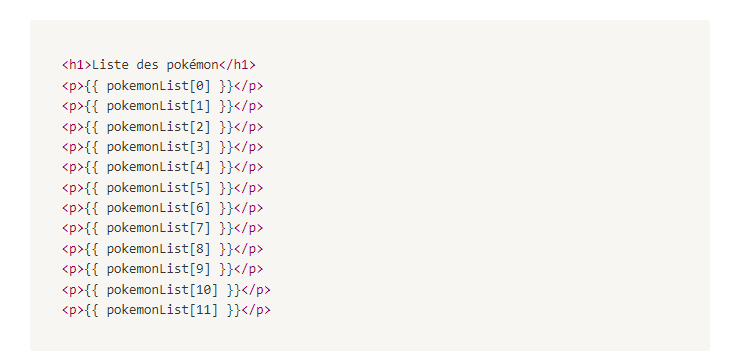
\includegraphics[width=14cm]{assets/inter} \newline


	\end{frame}

	\begin{frame}
		\frametitle{Template}

		Activité : \newline \newline

		- Regler le souci !

	\end{frame}

	\begin{frame}
		\frametitle{Template}

		L'interpolation : \newline

		\centering
		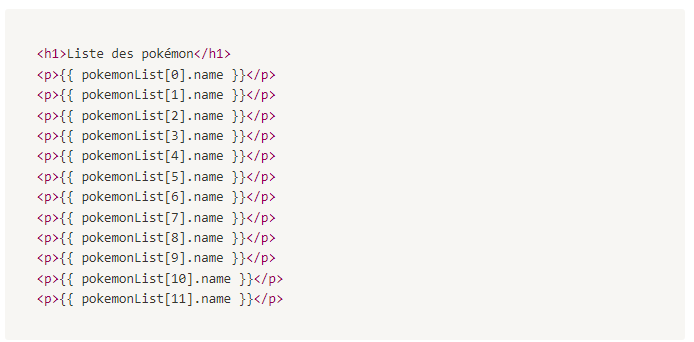
\includegraphics[width=14cm]{assets/inter2} \newline


	\end{frame}

	\begin{frame}
		\frametitle{Template}

		Activité : \newline \newline

		- Créé un tableau nommé "Personne" \newline
		- Dans ce tableau on aura un nom et un prénom et age \newline
		- Puis afficher dans le template avec la balise article le Nom, le Prenom et l'Age du tableau \newline \newline

		\centering
		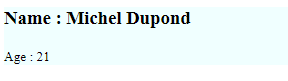
\includegraphics[width=8cm]{assets/exempleAct} \newline


	\end{frame}


	\begin{frame}
		\frametitle{Template}

		Interaction Utilisateur : \newline \newline

		Pour l’instant tout ce qu’on a vue c’est de trasmettre des donnée de la \alert{Logique} à la \alert{Vue} \newline \newline

		mais ce qu’on vas vouloir faire c’est l’inverse \newline \newline


		Donc ce qu’on vas vouloir faire : \newline
		C’est quand on clic sur un nom de pokemon  \newline excuter la fonction qu’on a créer “selectPokemon” \newline \newline


	\end{frame}

    \begin{frame}
        \frametitle{Template}

        Interaction Utilisateur : \newline \newline

        Donc comment on fait on vas simplement prendre un paragaphre d’un pokémon et on vas luis ajouter ceci \newline

        \centering
        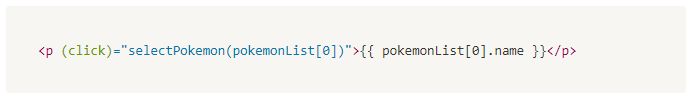
\includegraphics[width=14cm]{assets/interClick} \newline

    \end{frame}

	\begin{frame}
		\frametitle{Template}

		Interaction Utilisateur : \newline \newline

		On vas vouloir allez plus loin en créant un input qui envoie la donnée a notre fonction "showId" \newline

		\centering
		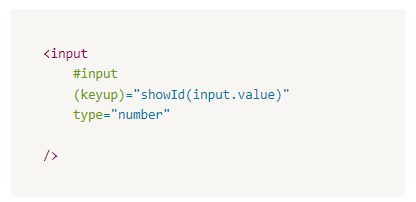
\includegraphics[width=8cm]{assets/input} \newline

		\begin{block}{Tips}
			En fesant (keyup.enter) la donnée s'envoie uniquement en cliquant sur la touche entré
		\end{block}

	\end{frame}

	\begin{frame}
		\frametitle{Template}

		Activité : \newline \newline

		Je veut quand je remplie le formulaire par un id : \newline
		- Que la console me sorte le nom du pokémon de cette id\newline
		- Et qu'il stock l'object de ce pokémon dans une nouvelle variable "pokemonSelected" \newline \newline

		\begin{block}{Information}
			Vous aurez besoin de créer une nouvelle fonction "showPokémon"
		\end{block}


	\end{frame}

	\begin{frame}
		\frametitle{Template}

		NgIf et NgFor : \newline \newline

		- NgIf permet d'effectuer une conditions dans le template \newline
		- NgFor permet de bouclé l'intergralité d'un tableau (foreach) \newline


	\end{frame}

	\begin{frame}
		\frametitle{Template}

		NgIf :

		On vas afficher un message différent si Salameche est trouver

		\centering
		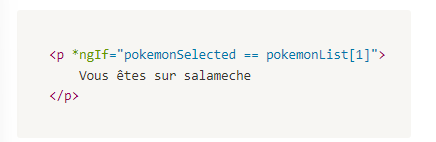
\includegraphics[width=8cm]{assets/ngif} \newline


	\end{frame}

	\begin{frame}
		\frametitle{Template}

		NgFor :

		On vas vouloir afficher tout les pokémon en quelque ligne

		\centering
		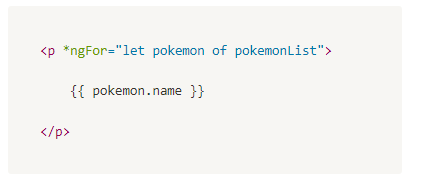
\includegraphics[width=8cm]{assets/ngfor} \newline


	\end{frame}

	\begin{frame}
		\frametitle{Template}

		Activité : \newline
		Je veut cette interface grace au ngFor \newline
		Et quand on click sur un pokémon je veut qu'il affiche le nom dans la console

		\centering
		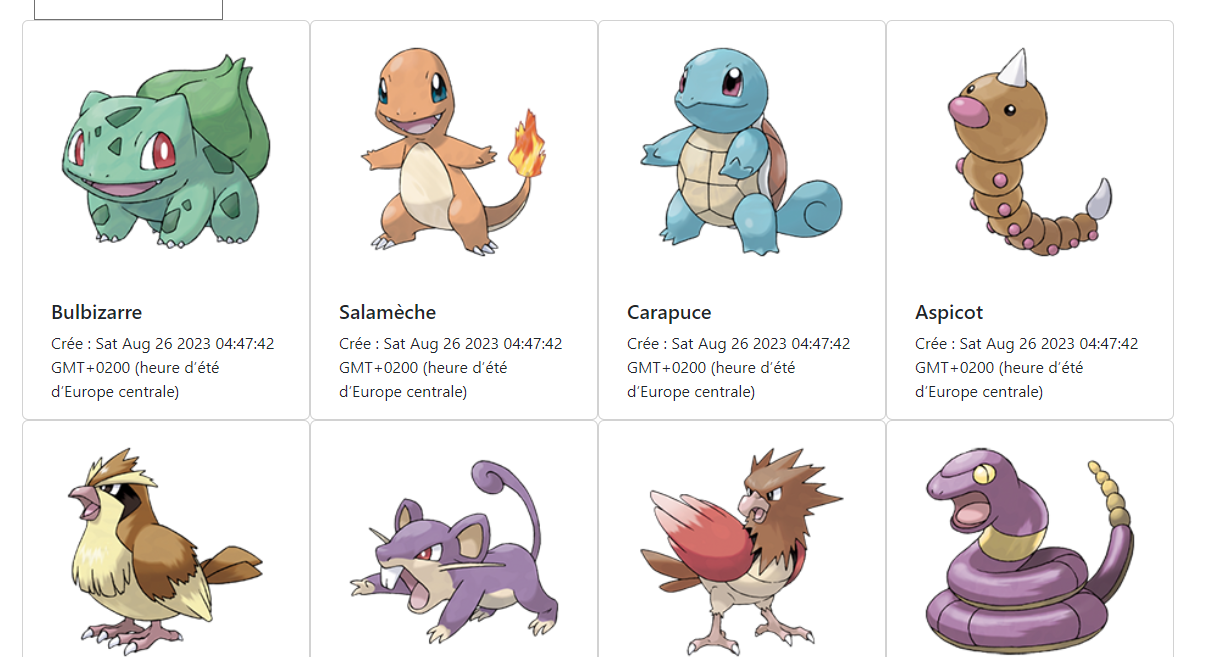
\includegraphics[width=9cm]{assets/allAct} \newline

		Utiliser Bootstrap

	\end{frame}

\end{document}